Intecs SpA com'è stato accennato nel capitolo introduttivo, ha sviluppato un sistema di certificazione della posizione basato su tecnologia GNSS/SDR. In questo capitolo daremo una panoramica del sistema di certificazione approfondendo le scelte implementative.

\section{Il sistema Galileo}
Prima di addentrarci nel progetto vero e proprio diamo maggiori dettagli sul sistema di posizionamento Galileo, utilizzato da Intecs SpA come sistema di posizionamento satellitare.

\subsection{Che cos'è Galileo?}
Il sistema di posizionamento Galileo è un sistema di posizionamento e navigazione satellitare civile, sviluppato in Europa come alternativa al Global Positioning System (NAVSTAR GPS), controllato invece dal Dipartimento della Difesa degli Stati Uniti d'America. Il sistema fornisce un grado di accuratezza di alcuni centimetri nelle tre direzioni, l'entrata in servizio inizialmente fu prevista a fine 2019 ma è stata poi anticipata al 15 dicembre 2016. Il sistema conta 30 satelliti artificiali orbitanti di cui 24 operativi più 6 di scorta.

\subsection{Storia}
I primi sistemi di posizionamento satellitare, furono sviluppati in piena guerra fredda per applicazioni militari e il loro utilizzo civile è ancora oggi, in linea di principio, subordinato alle necessità di impiego militare. La necessità di rompere il monopolio USA di un servizio su scala globale ha spinto l'Europa a varare il progetto Galileo.

\subsection{Principi di funzionamento}
Un sistema di posizionamento globale satellitare come Galileo è un sistema basato su una costellazione di satelliti artificiali in grado di fornire con estrema precisione le coordinate geografiche (longitudine, latitudine, quota)\footnote{La longitudine è la coordinata geografica che specifica quanto la posizione di un punto sulla superficie terrestre si trovi ad est oppure ad ovest rispetto al Meridiano di Greenwich assunto come riferimento. La latitudine è la coordinata geografica che specifica quanto la posizione di un punto sulla superficie terrestre si trovi a nord o a sud dell’equatore. L’altitudine o quota è la distanza verticale di un oggetto dal livello del mare, ossia l’altezza sul livello del mare.} e la velocità di qualsiasi mezzo fisso o mobile in ogni punto in prossimità della superficie Terra e nell'atmosfera, con continuità temporale. Ciascun satellite trasmette continuamente dei segnali codificati contenenti varie informazioni come i dati orbitali, che servono ad un ricevitore satellitare per il calcolo della posizione del satellite stesso e un riferimento temporale per la determinazione degli istanti esatti di trasmissione dei segnali stessi.

\subsection{Calcolo della posizione}
Il principio di funzionamento del sistema Galileo (e anche del GPS) è sostanzialmente semplice: si tratta di determinare la distanza da 4 satelliti (S1, S2, S3, S4) la cui posizione nello spazio è nota con precisione e, mediante opportuni passaggi matematici, determinare la propria posizione. Quando 4 satelliti sono misurati contemporaneamente, l’intersezione delle 4 sfere immaginarie individua la posizione del ricevitore [vedi figura \ref{fig: gps_triangolazione }]. Queste sfere si intersecheranno in parte invece che incontrarsi in un punto univoco e quindi il ricevitore calcolerà una approssimazione della posizione calcolata in modo probabilistico.
\begin{figure}[h]
\centering
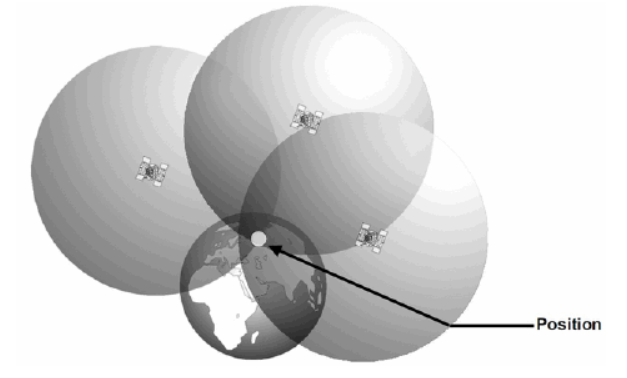
\includegraphics[scale=0.6]{images/gps_triangolazione.png}
\caption{Un esempio di triangolazione dei satelliti}
\label{fig: gps_triangolazione }
\end{figure}
La distanza del ricevitore dai satelliti viene determinata misurando lo scarto temporale che intercorre tra la trasmissione di una sequenza di bit inviata a Terra da ciascun satellite (trasmissione unidirezionale, tempi misurati da orologi atomici controllati e sincronizzati tra loro). Per utilizzare tale sistema in maniera unidirezionale, è necessario sapere con precisione l'istante di tempo in cui il codice viene trasmesso e misurare l'istante d'arrivo del segnale al ricevitore mediante l'uso di orologi esattamente sincronizzati. 

\subsection{Di cosa si occupa il sistema di certificazione realizzato da Intecs?}
Il sistema di certificazione della posizione verifica che lo snapshot registrato dal sistema mobile e dalla stazione di riferimento nello stesso momento sia equivalente. Se acquisiscono lo stesso snapshot, possiamo ipotizzare che nessuno stia cercando di attuare tecniche di spoofing e siamo in grado di considerare attendibile la posizione del dispositivo mobile, certificandolo. Sia il sistema mobile che la stazione di riferimento acquisiscono segnali da un certo numero di satelliti. Il confronto dei segnali viene eseguito su ogni satellite in comune cioè confrontando il segnale del solito satellite acquisito sia dal sistema mobile che dalla stazione di riferimento. Se alla fine del processo di confronto, un solo satellite in comune risulta non autenticato (cioè i due segnali sono diversi), la posizione non sarà certificata. In particolare, per poterla certificare è necessario che almeno quattro satelliti in comune siano autenticati. I segnali catturati dalla stazione di riferimento potrebbero essere "spoofati". Per risolvere questo problema si possono utilizzare più stazioni di riferimento per poter fare un check distribuito e su queste condizioni si considera totalmente sicura questa componente.

\section{Architettura del progetto iniziale}
L'architettura del sistema di certificazione della posizione realizzato da Intecs SpA è formata da tre componenti: sistema mobile, sistema centrale e stazione di riferimento. 
\begin{figure}[h]
\centering
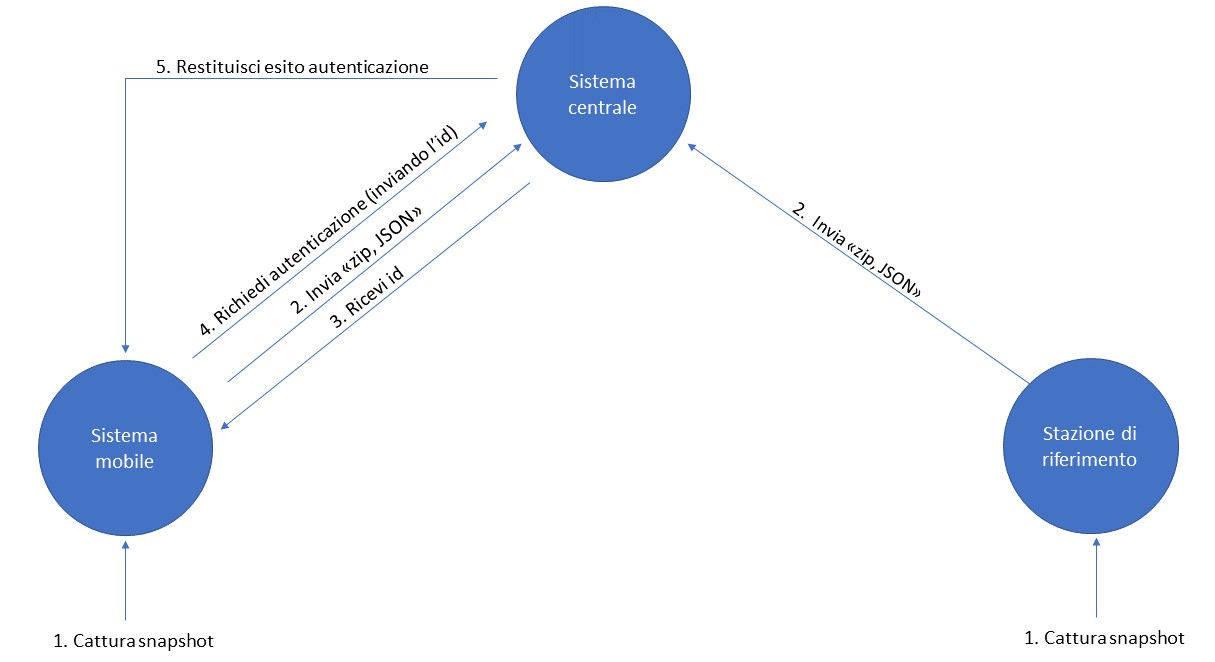
\includegraphics[scale=0.5]{images/schema progetto base.jpg}
\caption{Architettura del sistema di certificazione della posizione}
\label{fig: architetturabase }
\end{figure}
Sia il sistema mobile che la stazione di riferimento acquisiscono ogni 120 secondi\footnote{L'acquisizione dello snapshot può essere settato manualmente, ma non può essere mai inferiore ai 60 secondi.} un segnale\footnote{Questo tipo di segnale è rappresentato con una sequenza di bit.} da ognuno dei satelliti Galileo a cui si collegano, sfruttando un ricevitore satellitare. Lo snapshot catturato\footnote{Per semplicità chiameremo l'insieme di questi segnali acquisiti da un solo dispositivo (sistema mobile o stazione di riferimento) "snapshot".} viene salvato in un file all'interno di un archivio zip e utilizzato per calcolare i dati di posizione (altitudine, latitudine, longitudine ed altri parametri che per semplicità non considereremo) che assieme al timestamp sono inseriti in un file JSON. Il timestamp (o time-reference)\footnote{Un timestamp è una sequenza di caratteri che rappresentano una data e/o un orario per accertare l’effettivo avvenimento di un certo evento.} ha una precisione del millisecondo e rappresenta la data e l'ora dell'istante in cui il sistema mobile e la stazione di riferimento iniziano ad acquisire il segnale dai satelliti. Le due componenti sono sincronizzate con un orologio atomico in modo che la ricezione dello snapshot avvenga nel solito istante. L'acquisizione dello snapshot ha una durata di 5 secondi. Dopo la ricezione da parte del sistema mobile e dalla stazione di riferimento dello snapshot, entrambi inviano al sistema centrale due file rispettivamente: il file zip e il file JSON, attraverso una richiesta di tipo http-multipart\footnote{Una richiesta http-multipart è una richiesta http che i client http costruiscono per inviare file e dati su un server http.}. Il sistema mobile dopo l'invio dei due file, riceverà un messaggio di conferma ricezione contenente l'id univoco associato al file zip appena inviato, che utilizzerà per richiedere la certificazione dello snapshot al sistema centrale. A questo punto, il sistema centrale è in grado di verificare che i due snapshot siano uguali, comparandoli, il che significa confrontare ogni segnale (file binario) riferito al solito satellite in comune, sfruttando un algoritmo di allineamento delle due sequenze di bit. Questo allineamento è necessario visto che anche se gli snapshot vengono catturati dalle due macchine nello stesso istante e per lo stesso periodo di tempo (un intervallo di 5 secondi) gli orologi potrebbero non essere correttamente sincronizzati come in figura \ref{fig: algoritmoallineamento }]. In questo particolare esempio infatti, il sistema mobile inizia a catturare il segnale dal satellite Galileo "GSAT0103 - David" un istante prima rispetto a quello catturato dalla stazione di riferimento.
 \begin{figure}[h]
\centering
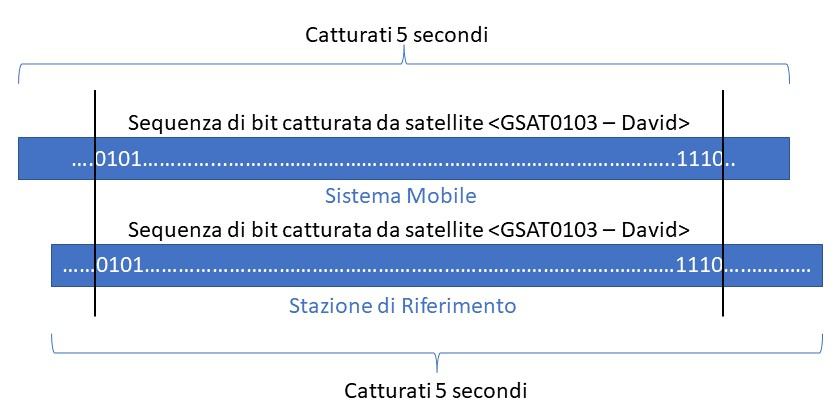
\includegraphics[scale=0.5]{images/grafico allineamento snapshot.jpg}
\caption{Un esempio di funzionamento dell'algoritmo di allineamento tra due snapshot}
\label{fig: algoritmoallineamento }
\end{figure}

\subsection{Database del Sistema Centrale}
Il sistema centrale ha due database interni: un Object Storage (gestito con MinIO\footnote{MinIO è un object storage le cui API sono compatibili con Amazon S3, un servizio offerto da Amazon Web Services (AWS) che fornisce storage di oggetti tramite un'interfaccia di servizio Web.}) che contiene gli snapshot e un database dei Metadati (gestito con Elasticsearch\footnote{Elasticsearch è un motore di ricerca e analisi dei dati distribuito basato su Apache Lucene.}) contenente i file JSON. Quando il sistema centrale riceve la richiesta http-multipart dal sistema mobile e dalla stazione di riferimento riceve sia il file zip che il JSON e inserisce il file zip (che contiene un file binario detto snapshot) nell'Object Storage. La procedura di inserimento restituisce un identificatore che rappresenta l'id univoco del file zip appena inserito nel database, questo file viene successivamente aggiunto ad un record assieme al file JSON e immagazzinato nel database dei metadati. La figura \ref{fig: salvataggioinfo } sottostante schematizza la spiegazione appena data.
\begin{figure}[!h]
\centering
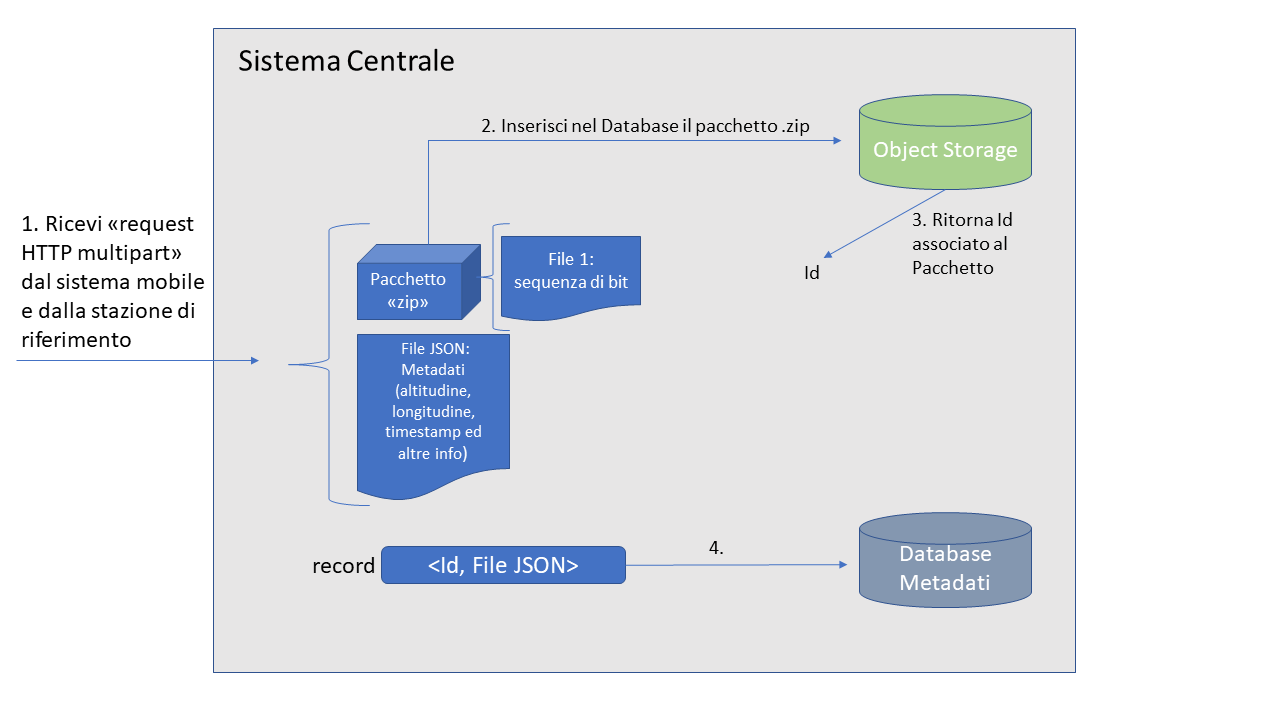
\includegraphics[scale=0.4]{images/Foto4.png}
\caption{Un esempio di salvataggio del file zip e del JSON}
\label{fig: salvataggioinfo }
\end{figure}

\subsection{Come confrontare gli snapshot}
Il confronto degli snapshot è un'operazione che avviene non appena il sistema centrale riceve dal sistema mobile la richiesta di autenticazione attraverso l'invio dell'id associato allo snapshot. Sfruttando l'id, il sistema centrale estrae il pacchetto zip nell'object storage e il record <id,json> dal proprio database dei metadati. Successivamente dal pacchetto zip viene estratto il file snapshot.bin. Si estrae il timestamp dal file JSON e si ricerca nel database dei metadati il record riferito alla stazione di riferimento. A questo punto viene confrontato, tramite l'algoritmo di allineamento degli snapshot visto sopra, lo snapshot del sistema mobile con quello della stazione di riferimento [vedi figura \ref{fig: ricercasnapshot }].
\begin{figure}[!h]
\centering
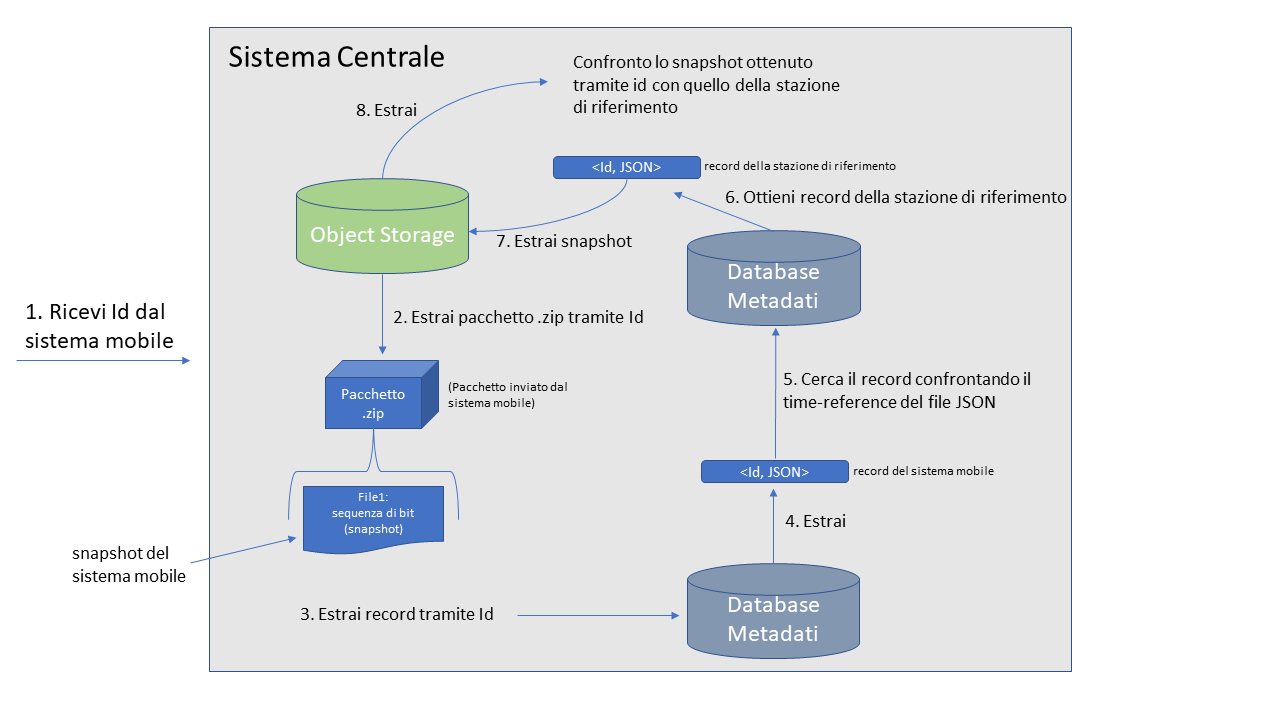
\includegraphics[scale=0.5]{images/Foto5.png}
\caption{Ricerca snapshot da id}
\label{fig: ricercasnapshot }
\end{figure}